\chapter{Technische Grundlagen} \label{Technische_Grundlagen}

\section{Internet Protocol Version 4 (IPv4)} \label{ipv4}
\subsection{Allgemeines und Adressierungsschema}
Das Internet Protocol ist im OSI-Modell auf Schicht 3 (Network-Layer) anzusiedeln. Es dient der \textit{Paketierung} von Daten und anschließenden Ende-zu-Ende-Vermittlung dieser \textit{Pakete} zwischen Netzwerk-Systemen. Dafür notwendig ist eine Adressierung: eine IPv4-Adresse besteht aus einer 32 Bit-Zahl, welche typischerweise dezimal dargestellt wird in so genannter \glqq dotted decimal\grqq{}-Schreibweise. Dafür wird die Binärzahl in vier Oktette mit einem Punkt aufgeteilt und die jeweiligen Oktette in dezimal umgerechnet.

00000001000000100000001100000100 (32-Bit Integer) ->  00000001.00000010.00000011.00000100 (dotted binary) -> 1.2.3.4 (dotted decimal)

Mit Hilfe von Netzmasken wird die Netzwerkgröße bestimmt. Der Host mit der IP-Adresse 1.2.3.4 und einer Netzmaske von bspw. 255.255.255.0. Diese Netzmaske entspricht in dotted binary:

11111111.11111111.11111111.00000000

Die ersten 24 Bit sind für das Netzwerk reserviert (Network bits), die letzte 8 Bit sind Host bits. Dieses Netzwerk kann somit theoretisch aus $2^8 = 256$ Hosts bestehen, wobei die erste und letzte Adresse reserviert sind (Netzwerkadresse und Broadcast-Adresse).

Heutzutage üblich ist die so genannte CIDR-Notation, welche IP-Addresse und Subnetzmaske vereint. Wenn man die erwähnten Beispiele aus Adresse und Subnetzmaske zusammenführt, erhält man die IP-Adresse in CIDR-Notation: 1.2.3.4/24. /24 entspricht dabei den gesetzten Network bits.

Mit Hilfe der IP-Adresse und Netzmaske lässt sich ermitteln, ob sich ein Host im gleichen \textit{Subnetz} befindet. Dafür berechnet man die Netzwerkadresse per logisch-AND:

\begin{lstlisting}[label=local-ip-address-AND-subnet,caption=Blub]
    00000001.00000010.00000011.00000100
AND 11111111.11111111.11111111.00000000
    00000001.00000010.00000011.00000000 => Netzwerkadresse: 1.2.3.0/24
\end{lstlisting}
    
Hat man nun zwei Hosts 1.2.3.240 und 8.9.10.23, mit denen man eine IP-Verbindung aufbauen will, so prüft der Initiator zuerst, ob das jeweilige Netz \textit{link-lokal} erreichbar ist, also im gleichen IP-Netzwerk wie der Initiator liegt.

Für 1.2.3.240:

\begin{lstlisting}[label=local-ip-address-AND-subnet-same,caption=Blun]
... 00000001.00000010.00000011.11110000
AND 11111111.11111111.11111111.00000000
  = 00000001.00000010.00000011.00000000 => Netzwerkadresse: 1.2.3.0/24 (gleiche Netzwerkadresse wie oben, link-lokal erreichbar)
\end{lstlisting}

Für 8.9.10.23:

\begin{lstlisting}[label=local-ip-address-AND-subnet-different,caption=Blub]
    00001000.00001001.00001010.00010111
AND 11111111.11111111.11111111.00000000
    00001000.00001001.00001010.00010111 => Netzwerkadresse: 8.9.10.0/24 (andere Netzwerkadresse: das Paket muss \textit{geroutet} werden)
\end{lstlisting}

\subsection{RFC 1918-Adressen}
%https://datatracker.ietf.org/doc/html/rfc1918
Ein Großteil der IP-Adressen werden \textit{blockweise} an Provider, Firmen und Forschungseinrichtungen herausgegeben und können fortan im Internet genutzt werden. Mit RFC 1918  wurden Blöcke durch die IANA reserviert, welche ausschließliche für private und firmeninterne Nutzung vorgesehen sind. Sie werden im Internet nicht geroutet. Es handelt sich dabei um die Blöcke:
\begin{itemize}
\item 10.0.0.0/8
\item 172.16.0.0/12
\item 192.168.0.0/16
\end{itemize}

Auf diese Blöcke wird auch in der Bachelor-Arbeit zurückgegriffen, um Zugriff auf \textit{interne}, vom Internet \textit{isolierte} Ressourcen zu ermöglichen.

\subsection{IP-Routing}

Wie im vorherigen Beispiel gefolgert, müssen Pakete, die Ziele in anderen Subnetzen haben, geroutet werden. Dafür besitzen alle Netzwerkteilnehmer eine Routing-Tabelle, um herauszufinden, an welchen \glqq Next-Hop\grqq{} ein Paket adressiert werden muss. Im folgenden Beispiel besteht das Netzwerk aus vier Teilnehmern: einem Client, einem Server und zwei Routern (R1 und R2). Alle Geräte verwalten eine Routing-Tabelle, in denen die Zielnetze und Next-Hops vermerkt sind. Damit weiß der Client, dass Pakete für das Netzwerk 192.168.200.0/24 über R1 mit der IP-Adresse 192.168.0.1 geschickt werden müssen. R1 nimmt das Paket an, schaut wiederum in der eigenen Routing-Tabelle nach und schickt das Paket dann weiter an R2, usw. (Rück-)Pakete vom Server zum Client durchlaufen die gleiche Prozedur pro Hop. Client und Server müssen im Übrigen das Netzwerk 192.168.100.0/30 \textbf{nicht} in ihrer Routing-Tabelle pflegen. Dieses Netzwerk hat eine ausschließliche Relevanz zur Übertragung von Daten zwischen R1 und R2: Man spricht auch von Transfernetzwerken.\\

\begin{figure}[h]
  \centering
  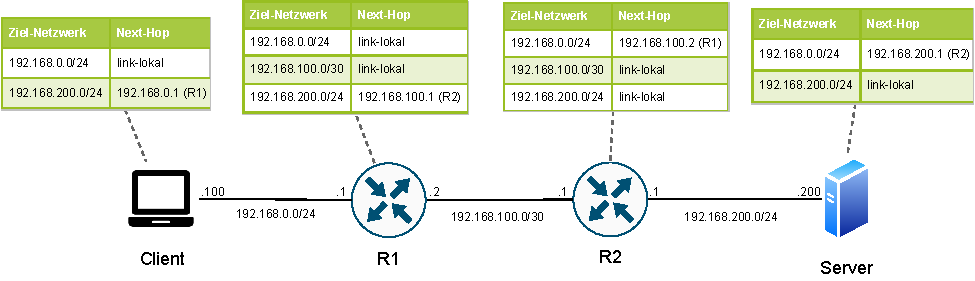
\includegraphics{Figures/next_hop_routing_specific_table.pdf}
  \caption{Next Hop Routing}
  \label{grafik: next_hop_routing}
\end{figure}

Dieses Beispiel bringt ein Skalierungsproblem mit sich: Umso mehr Subnetze existieren, in denen Server zu erreichen sind, desto mehr Routen muss der Client in der Routing-Tabelle (manuell) pflegen. Das gleiche gilt für Server, insofern eine Server-zu-Server-Kommunikation gewünscht ist.
In der Praxis sieht man kaum noch Endsysteme (darunter fallen Client und Server), welche mit solchen \textit{spezifischen} Routen arbeiten. Man überlässt die komplexe Verwaltung von Routing-Tabellen den Routern, während die Endsysteme neben der link-lokalen nur noch die \textit{Default}-Route besitzen. In diese Route 0.0.0.0/0 fallen alle Zielnetzwerke, abgesehen vom link-lokalen Subnetz, und sie zeigt immer auf den lokal erreichbaren Router.\\
Das Setzen der Default Route garantiert allerdings nicht, dass ein Ziel auch wirklich erreicht werden kann, z.B. weil es gar nicht existiert oder das Zielnetzwerk nicht in der Routing-Tabelle eines (Next-Hop-)Routers vorhanden ist. Ein Hilfsprotokoll zur Signalisierung von Erreichbarkeit ist dabei das Internet Control Message Protocol (ICMP). Das bekannte Werkzeug Ping nutzt Nachrichten in Form von ICMP Echo Request und ICMP Echo Response, um die Erreichbarkeit eines Endsystems zu prüfen.
\begin{figure}[h]
  \centering
  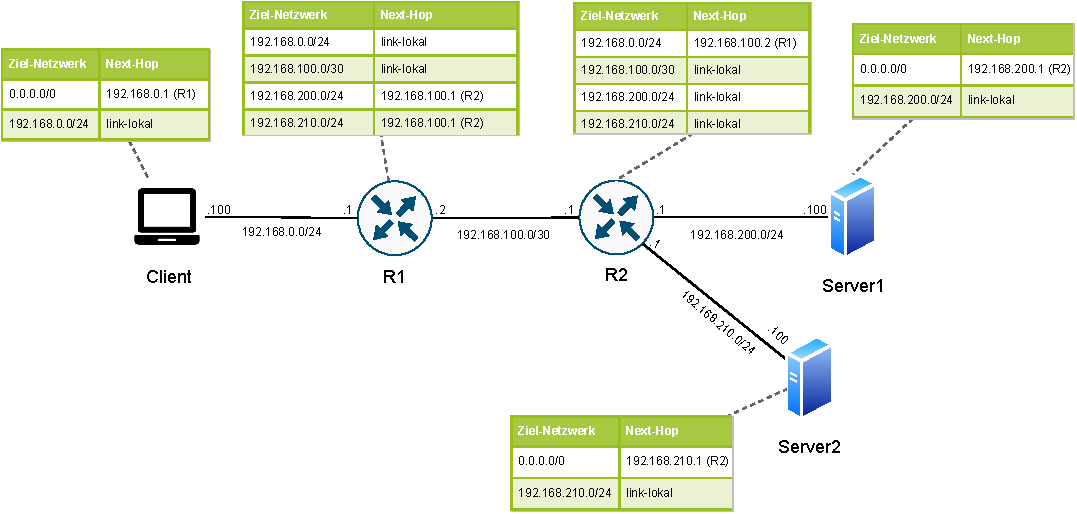
\includegraphics{Figures/next_hop_routing_default_route.pdf}
  \caption{Next Hop Routing mit Default Route}
  \label{grafik: next_hop_routing_with_default_route}
\end{figure}\FloatBarrier




Prinzipiell spielen im IPv4-Routing viele weitere Mechanismen eine zentrale Rolle: Zu nennen wären an dieser Stelle bspw. MAC-Adressen (Ethernet), Address Resolution Protocol (ARP), Metrik und Time-To-Live (TTL). Für diese Ausarbeitung haben die Themen allerdings keine Relevanz. Das Thema \glqq dynamisches Routing\grqq{} wird später noch behandelt.
%Transfernetzwerk
%keine Metrik / AD
%In den Ursprüngen des Internets waren IP-Adressen \textit{classful}: die Netzwerkgröße wurde über die Klassenzugehörigkeit einer IP-Adresse bestimmt. Ein Class A Netz fiel in die \textit{Range} 0.0.0.0 - 127.255.255.255. So hätte obige IP-Adresse zu dem Class-A-Netzwerk "1.0.0.0" gehört